\section{Introduction}
\label{sec:introduction}

%Recent years have witnessed a rapid adoption of 
Internet-of-Things (IoT) technologies are being rapidly adopted in the consumer electronics market.
There has been increasing deployment of ``smart'' devices in the home environment to create interactive, ``human-in-the-loop'' applications and services.
In addition to their use in traditional home automation systems, IoT technologies have also been applied to home entertainment--for example, with wireless inertial sensors used to track user body movement in sports games. Combined with emerging virtual and augmented reality technologies, IoT offers the promise of new immersive and interactive experience for end-users.
Common requirements for such systems include:
\begin{itemize}
\item Integration of heterogeneous devices and services from different vendors;
\item Interactive user experience that emphasize real-time feedback loop;
\item Easy installation and configuration; and
\item Security protection, due to tight integration with the home network.
\end{itemize}

Many IoT frameworks and ecosystems~\cite{alljoyn,iotivity,aws-iot,weave,azure-iot,smartthings,homekit} have been proposed over the last few years to facilitate the development of more sophisticated applications like these.
They typically provide a similar set of framework-level services, including user and device authentication and authorization, device and service discovery, device management, publish-subscribe messaging, and remote access.
On top of these common services, IoT developers can further design and implement application-specific functionality. % such as monitoring, automation, storage, machine learning, and integration with external systems.
Fig.~\ref{fig:service-arch} shows a common hierarchical architecture of IoT services, where ``named entities'' refer to users, devices, and applications that require trust management and utilize rendezvous services to get organized into a coherent home IoT system.

\begin{figure}[!t]
\centering
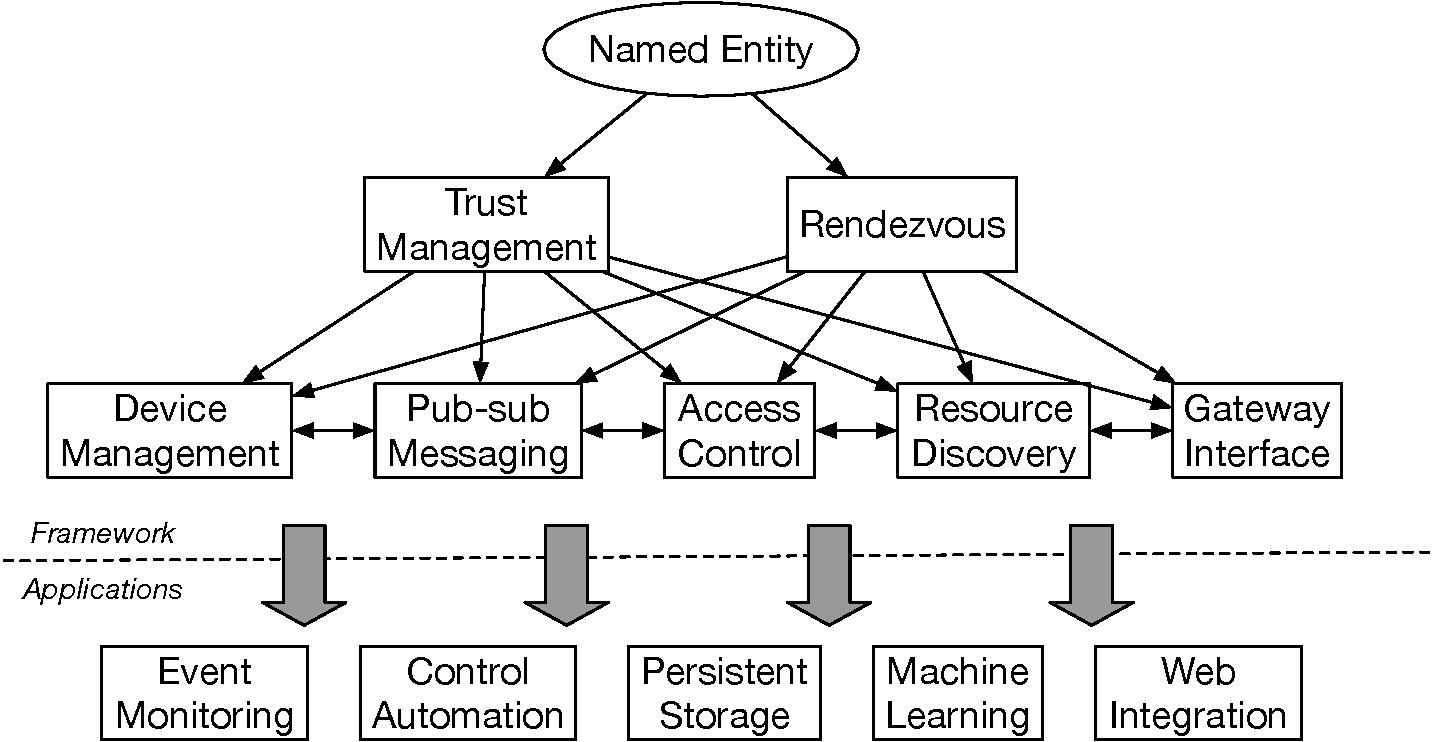
\includegraphics[width=0.95\columnwidth]{service-arch.pdf}
\caption{Hierarchical architecture of IoT services.}
\label{fig:service-arch}
\end{figure}

Existing home IoT systems often depend on cloud-based services provided by device vendors and/or service providers to implement both the framework services and application functions needed in local IoT communication.%
%The cloud-based solutions leverage remote services to manage trust and rendezvous, from which other services and applications (both locally and in the cloud) can be bootstrapped.
\footnote{Cloud services also support features, such as voice recognition, which are difficult to achieve locally; such services are not foundational to IoT communications and thus not our focus here.}
Such dependency on the cloud, for what could be inherently local functionality, introduces limitations including:
\begin{itemize}
\item The home IoT system requires cloud connectivity to manage local devices and users; the user cannot install new devices or authorize new users if connection to the cloud is lost or even intermittent.

\item Cloud-based services expose data from the home environment to external parties, introducing potential security and privacy risks.
 
\item With cloud-based services, 
% For devices that are connected directly to the Internet, 
the control and resource access commands have to go through the cloud that acts as the rendezvous point, even if the command issuer may reside in the same local network with the target device.\footnote{Even when a local IoT hub is deployed, the remote commands originated outside the home network still have to be tunneled through the cloud for NAT traversal.}
%% LZ: not sure what this footnote means...
This introduces additional delays that may hurt interactive applications.
\end{itemize}

This paper presents an alternative approach based on the Named Data Networking (NDN) architecture~\cite{ccn-van,ndn}, which focuses on enabling these functions to be achieved locally first, with cloud connectivity optional.  It builds on our previous work in~\cite{ndn-iot} to develop a specific design and implementation for how the foundational functions of \emph{trust management} and \emph{rendezvous}, shown in in Figure~\ref{fig:service-arch}, can be built up from NDN primitives. 

In Section~\ref{sec:background}, we first give an overview of representative IoT ecosystems and outline their dependencies on the cloud. 
We then describe in more detail these two foundational IoT services, trust management and rendezvous, which provide the basis for bootstrapping other services.  We show that both of them can be supported more efficiently in IoT networks under the Named Data Networking architecture (Section~\ref{sec:ndn-iot}). 
The key idea behind such a cloud-independent architecture design is to leverage NDN's named-based forwarding to directly operate on well-established naming in the local context.  This enables straightforward solutions for trust management, via schematized trust, and rendezvous, via distributed dataset synchronization.

In Sections~\ref{sec:components} and~\ref{sec:implementation}, we present the design and implementation of Flow, an IoT-augmented home entertainment experience, as a realization of the proposed IoT approach using NDN. 
While this implementation focuses on an interactive home entertainment application, we believe that our approach also applies to traditional home automation systems and many other IoT subdomains. We conclude with a brief comparison of how Flow could be achieved on Apple HomeKit and AWS IoT services, two popular TCP/IP-based IoT frameworks.
